\documentclass{article}
\title{CS 279 Assignment 2: Conduct an Experiment\\Part 3: Online study and data analysis}
\author{Miriam Cha and Melih Elibol}
\date{September 30, 2014}

\usepackage{amsmath}
\usepackage{bbm}
\usepackage{fullpage}
\usepackage{graphicx}
\usepackage{listings}
\usepackage[usenames,dvipsnames]{color}

\usepackage{amsmath,graphicx,amssymb,amsfonts,bbm,subfigure}
\usepackage{array,colortbl,xcolor}

\usepackage{tikz}
\usetikzlibrary{shapes,arrows}
\usepackage{caption}

\begin{document}
\maketitle

In this report, we emulate the experimental process Study 2 in Scarr. J., et al (2012). The authors compare two interfaces: CommandMap and Microsoft's Ribbon. Using the interfaces, Study 2 tests the following hypotheses:
\\
\noindent 
\textbf{H1}: Knowledgeable users can select commands faster using CommandMaps than when using Ribbons.\\
\textbf{H2}: CommandMaps are faster than the Ribbon for tasks requiring switching between different parent tabs.\\
\textbf{H3}: Users will prefer CommandMaps over Ribbon. 

Beyond emulation, we have extended Study 2 to include online as well as offline participants. This report includes observation, analysis, and discussion for our study. The organization for the remainder of the report is as follows: In Section 1, we provide detailed procedures, participant demographics, design specifications, and analysis of offline and online tests. Section 2 contains experimental results based on statistical analysis, and Section 3 concludes the report with interpretations and discussions of the results. 

\section*{1. Design and Analysis}
We designed our study with an offline population and two online populations: participants recruited via Amazon Mechanical Turk and unpaid volunteers recruited via our own social networks. The compatibility of our website is tested with the latest versions of Chrome, Safari, and Firefox. 
\\

\noindent
\textbf{Laboratory Study}: Ten participants were recruited from Harvard University. The experiment were conducted on a 20'' screen, running at a resolution of 1680x1050, same location, and time period (4pm-7pm).\\

\noindent\textbf{Online Study}: 10 participants were recruited from Mechanical Turk and 32 participants were recruited from our own social networks. For both populations, we provided the following instructions: Please open this url in a browser other than IE and maximize your screen. You will be given further instructions upon clicking the start button below; Please maximize your screen and carry out subsequent instructions as quickly as possible. 

During offline testings, we observed that our experiment took approximately five to ten minutes, so we relaxed the time range of our experiment to ten minutes per a HIT and paid Turkers \$1/HIT ($\approx$\$6/1hr). In order to prohibit multiple plays by the same Turkers, we designed our website to check `localStorage' to verify that the Turkers have not previously participated in the experiment. At the end of each experiment, we presented unique session ID and ask Turkers to insert the ID as a survey code. 

\section*{2. Results} 
We analyzed task time, error, and survey data for CommandMap and Ribbon with and without trials containing tab switches. Lab-based and online-based data are separately presented.
\subsection*{Laboratory Study}
Mean acquisition times were faster with CommandMap (1.13 s, s.d. 0.6) than Ribbon (1.69 s, s.d. 1.27). \textit{T-test} confirms that the difference in mean selection time between CommandMap and Ribbon is significant, giving $p<0.001$. We therefore find support for \textbf{H1}.

%$F = 5.11, p<0.05$. Bonferroni corrected pairwise comparisons confirms that the differences in mean selection time between CommandMap and Ribbon is significant. A 95$\%$ confidence interval for the difference is $[-1.06, -0.06]$, which means we can reject the hypothesis that the true difference is zero. This is also confirmed by the corresponding p-value of 0.03.

Mean acquisition times with same parent were faster than with different parent for both CommandMap and Ribbon. As shown in Figure~\ref{fig:result1}(a), the average acquisition time for CommandMap with same parent was $0.7$ seconds and with different parent was $1.56$ seconds. Similarly, the average acquisition time for Ribbon with same parent was faster than the time with different parent. Our analysis showed that CommandMap and Ribbon with same parent are not too different from each other ($p<0.5$). Additionally, we showed that CommandMap and Ribbon with different parents are significantly different from each other ($p<0.001$). As a result, we concluded that CommandMap performed similarly for same parent, but CommandMap was faster than Ribbon for different parent. We therefore find support for \textbf{H2}. 

Figure~\ref{fig:result1}(b) shows mean error rate (total number of miss clicks/total clicks) with error bar showing standard error. Error rates for CommandMap vs. Ribbon with same or different parent were not too different from each other ($p<0.5$). However, CommandMap had lower mean error than Ribbon for both same and different parent. Again, this observation aligns with the finding in the original paper. Our results showed that tab switch has an effect in CommandMap, yielding some slope in Figure~\ref{fig:result1}(a). By visual inspection, our slope is considerably larger than the one presented in Figure5(a) in the original paper. We suspect this is due to not centering the cursor for each trials in our CommandMap study. Even though this issue was discussed in Part 2, we intentionally kept this setting to have consistent experimental setup between offline and online experiments. 

User response to CommandMap was more favorable than Ribbon. With 10 participants, 7 rated CommandMap as their preferred interface. We therefore find support for \textbf{H3}.CommandMap was rated as having the lowest workload on all significant NASA-TLX measures except for Temporal demand (See Table~\ref{fig:trial_log}). 

\begin{figure}[tbh]
    \centering
    \subfigure[Task time]
    {
    %left, bottom, right, top%
    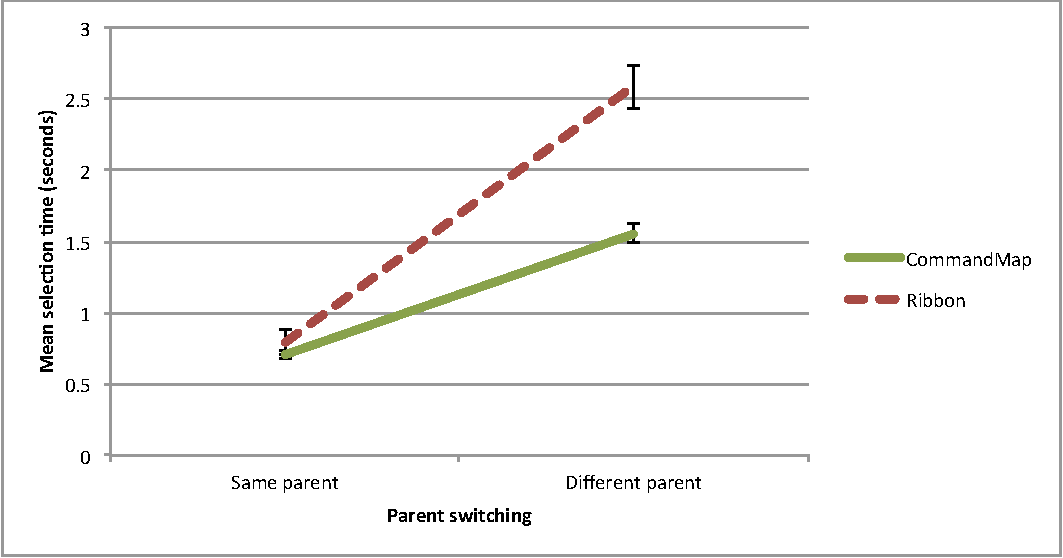
\includegraphics[trim = 0mm 0mm 0mm 0mm, clip,width=80mm]{figure5a_stderr.pdf}
    }
    \subfigure[Errors]
    {
    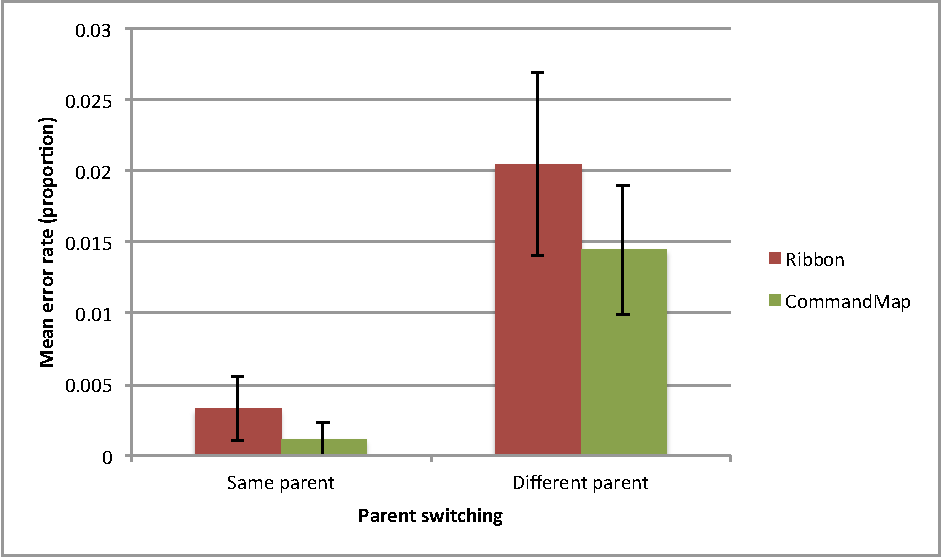
\includegraphics[trim = 0mm 0mm 0mm 0mm, clip,width=70mm]{figure5b_stderr.pdf}
    }
    \caption{Offline results for Study 2, with (a) shown as a line chart and (b) shown as a bar chart for consistency with Figure 5 in the original paper. Error bars show standard error.}
    \label{fig:result1}
\end{figure}

 \begin{table}[tbh]
  \centering
\begin{tabular}{c|c|c|c|c}
  &  \textbf{Ribbon}  &  \textbf{CM} &  \textbf{$\chi^2$} & \textbf{Sig}          \\\hline
 \textbf{Mental demand}&   2.7 (1.2)  & 2.2 (1.2)  & 16.7  & $<0.06$   \\ \hline
 \rowcolor{lightgray}
\textbf{Physical demand}  &    1.9 (1.2) &   1.5 (0.5) & 4.1  & $<0.2$  \\\hline       
\textbf{Temporal demand}  &    3.2 (1.1) &   3.3 (1.0) & 22.4  & $<0.04$  \\\hline      
 \rowcolor{lightgray}
\textbf{Hard work}  &    2.8 (1.1) &   2.7 (1.1) & 20.0  & $<0.02$   \\\hline   
\textbf{Frustration}  &    1.9 (0.7) &   1.5 (0.7) & 7.3  & $<0.2$ \\ \hline \hline
\end{tabular}
\caption{Mean (st. dev.) NASA-TLX values (1=low, 5=high)}
\label{fig:trial_log}
\end{table}




\subsection*{Online Study}
Mean acquisition times were faster with CommandMap (1.35 s, s.d. 0.6) than Ribbon (1.99 s, s.d. 1.26). \textit{T-test} confirms that the difference in mean selection time between CommandMap and Ribbon is significant, giving $p<0.001$. We therefore find support for \textbf{H1}.

As shown in Figure~\ref{fig:result2}(a), mean acquisition times with same parent were faster than with different parent for both CommandMap and Ribbon. Our analysis showed that CommandMap and Ribbon with same parent are not too different from each other ($p<0.1$). However, we showed that CommandMap and Ribbon with different parents are significantly different from each other ($p<0.001$). As a result, we concluded that CommandMap performed similarly for same parent, but CommandMap was faster than Ribbon for different parent. We therefore find support for \textbf{H2}. 

For online data collection, we observe higher mean error rate for CommandMap than Ribbon with both same parent and different parent. From Table~\ref{fig:trial_log2}, we see that the CommandMap bars (green) are consistently higher than the Ribbon bars (red), but the p-values that compare CM vs Ribbon with same parent and different parent are $p<0.8$ and $p<0.5$, respectively. Therefore we consider the higher error rate for CommandMap as a significant effect. 

\begin{figure}[tbh]
    \centering
    \subfigure[Task time]
    {
    %left, bottom, right, top%
    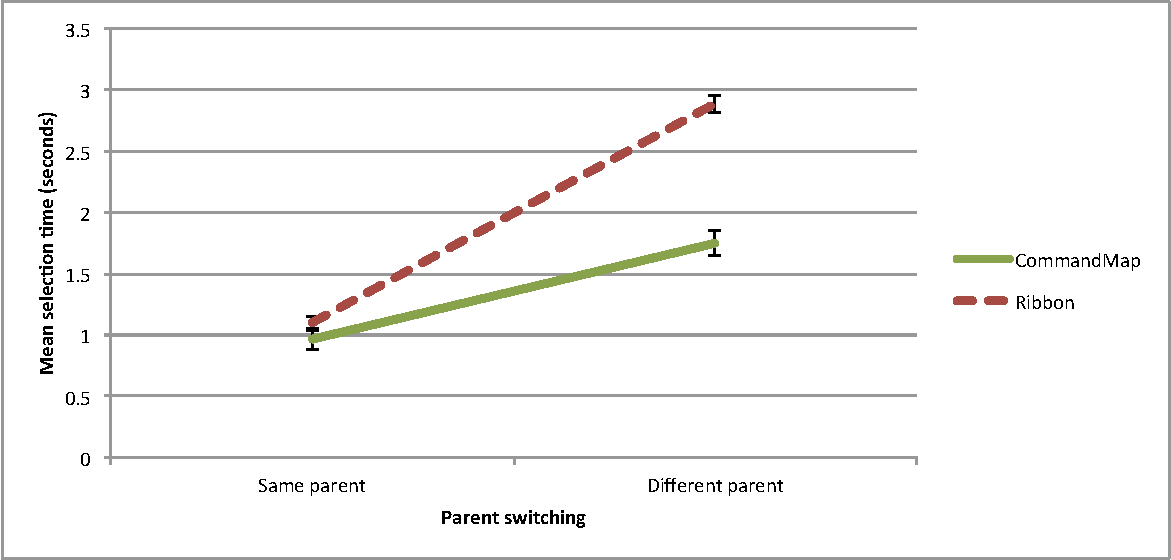
\includegraphics[trim = 0mm 0mm 0mm 0mm, clip,width=74mm]{figure5a_stderr_online.pdf}
    }
    \subfigure[Errors]
    {
    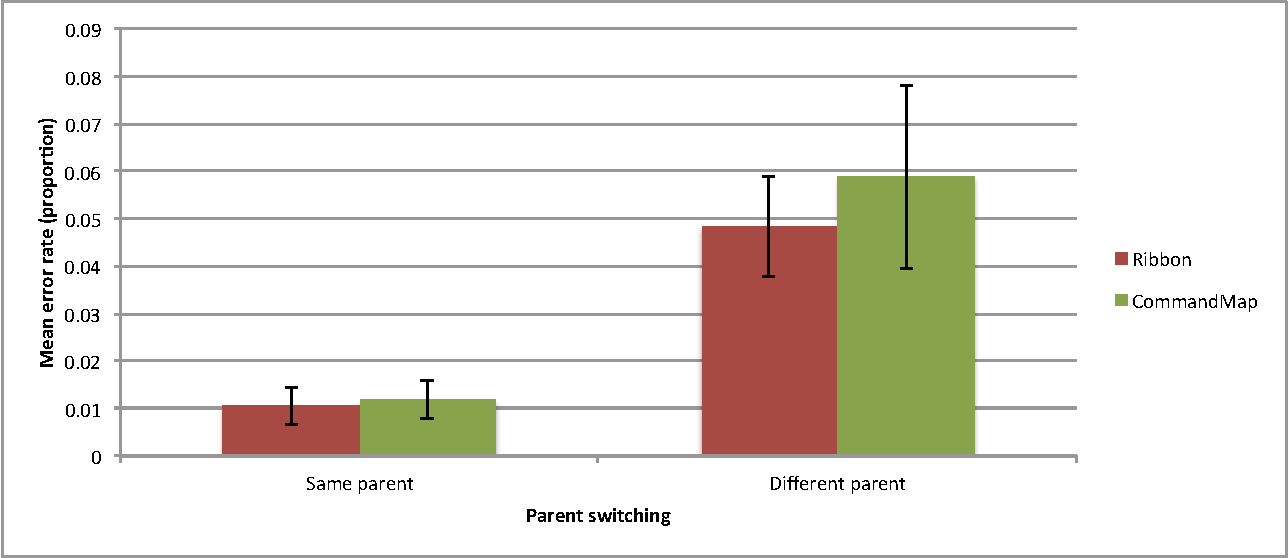
\includegraphics[trim = 0mm 0mm 0mm 0mm, clip,width=81mm]{figure5b_stderr_online.pdf}
    }
    \caption{Online results for Study 2, with (a) shown as a line chart and (b) shown as a bar chart for consistency with Figure 5 in the original paper. Error bars show standard error.}
    \label{fig:result2}
\end{figure}

 \begin{table}[tbh]
  \centering
\begin{tabular}{c|c|c|c|c}
  &  \textbf{Ribbon}  &  \textbf{CM} &  \textbf{$\chi^2$} & \textbf{Sig}          \\\hline
 \textbf{Mental demand}&   2.5 (1.1)  & 2.2 (1.0)  & 12.7  & $<0.4$   \\ \hline
 \rowcolor{lightgray}
\textbf{Physical demand}  &    2.4 (1.1) &   2.1 (1.2) & 24.8  & $<0.08$  \\\hline       
\textbf{Temporal demand}  &    3.1 (1.1) &   2.9 (1.2) & 15.2  & $<0.5$  \\\hline      
 \rowcolor{lightgray}
\textbf{Hard work}  &    2.7 (1.1) &   2.7 (1.1) & 13.5  & $<0.7$   \\\hline   
\textbf{Frustration}  &    3.1 (1.3) &   2.6 (1.4) & 19.7  & $<0.3$ \\ \hline \hline
\end{tabular}
\caption{Mean (st. dev.) NASA-TLX values (1=low, 5=high)}
\label{fig:trial_log2}
\end{table}

Unlike offline testing, user response to CommandMap was not necessarily favorable than Ribbon. With 42 participants, 20 rated CommandMap as their preferred interface. This result does not support \textbf{H3}. However, CommandMap was rated as having the lowest workload on all significant NASA-TLX measure. This result aligns with the result of the original paper. 


\section*{3. Discussion} 
\subsection*{Laboratory Study}
To summarize lab-based results, our study confirmed that users can select items more efficiently (faster speed) and effectively (less error) when the items are presented with flat hierarchy. Efficiency of flat hierarchy is well supported in our experiment. However, it is hard to make as strong of a statement on effectiveness as we observed overlapping standard error bars in Figure~\ref{fig:result1}(b). We suspect this is due to not having enough samples in our experiment. 

%Similar to Study 2 results in the paper, our experimental results show that CommandMap and Ribbon with same parent are not too different from each other ($p<0.5$). Additionally, we showed that CommandMap and Ribbon with different parents are significantly different from each other ($p<0.001$). This analysis aligns with the results in Study 2.  

%However our results show that tab switch has an effect in CommandMap, yielding some slope in Figure~\ref{fig:result1}(a). By visual inspection, our slope is considerably larger than the one presented in Figure5(a) in the paper. We suspect this is due to not centering the cursor for each trials in our CommandMap study. Even though this issue was discussed in Part 2, we intentionally kept this setting consistent to control the dependent variable. 

The original paper claims that ``CommandMap error rates are relatively unaffected by parent, while ribbon has much higher errors in different parent tasks.'' However our results show that CommandMap error rates are relatively affected by parent. We argue that this difference is caused by `temporal demand' of our participants. For all columns in Table~\ref{fig:trial_log}, Ribbon came out to have lower demand than CommandMap except for `Temporal demand.' Intuitively, participants are prone to make more errors if they are rushed to complete tasks. It is unclear why participants were more rushed to complete CommandMap than Ribbon. 

\subsection*{Online Study}
Our online study shows that knowledgeable users can select commands faster using CommandMaps than when using Ribbons (\textbf{H1}) and CommandMaps are faster than the Ribbon for tasks requiring switching between different parent tabs (\textbf{H2}). However, the online study fails to find support for \textbf{H3}.

Another interesting result that is different from results from both the offline and the original study is error analysis. Although \textit{T-test} confirms that this discrepancy is insignificant, it is still of our interest to find a reason for higher error rate of CommandMap than Ribbon. We suspect that smaller monitor size could affect the error rate of CommandMap because participants need to scroll up and down in order to select command targets. This frequent scrolling can cause more misclicks in CommandMap than Ribbon, does not require scrolling. 

\pagebreak

\end{document}
